\chapter{Implementation and Empirical Evaluation}

\section{Technology and Environment}
For the experimental verification, Python 3.x \cite{python3} was selected primarily to integrate seamlessly with the open-source \texttt{string-algorithms} repository. Despite Python being an interpreted language, its native support for very large integers is absolutely critical for executing the classical Fischer-Paterson bitwise algorithm optimally without dealing with artificial byte-overflows. Fast Fourier Transforms and discrete convolutions were executed using the SciPy library \cite{scipy2020}. 

To maximize operational performance, SciPy uses C/C++ internally, which makes array operations much faster and bypasses standard Python limitations. This allows the convolution operations to run at near-native speeds.

It is worth noting that Indyk's algorithm \cite{indyk1998} theoretically achieves an $\mathcal{O}(n \log n)$ time complexity using $GF(2)$ arithmetic. However, our implementation uses SciPy's FFT convolutions, which increases the complexity to $\mathcal{O}(n \log^2 n)$. This trade-off maintains consistency with the rest of the codebase, avoids slow bit-level operations in Python, and leverages optimized C routines.

A similar practical trade-off applies to the Kalai and Clifford-Clifford algorithms. To achieve their optimal $\mathcal{O}(n \log m)$ theoretical complexity, the text must be divided into smaller overlapping chunks. However, our implementation processes the entire sequence at once. While this single global FFT convolution changes the theoretical time to $\mathcal{O}(n \log n)$, it avoids the overhead of managing multiple block boundaries. Processing one large array allows the code to fully rely on SciPy's optimized C-backend.

\subsection{Handling Floating-Point Errors}
Because FFT uses complex numbers and floating-point arithmetic (IEEE 754 standard) \cite{chapra2015}, it naturally introduces small rounding errors during calculations.

In exact mathematics, a perfect match evaluates to exactly zero. However, in floating-point arithmetic, computed values might exhibit a tiny residual drift, typically ending up as something like $10^{-14}$. Because of this, direct boolean comparison (checking if \texttt{y == 0}) is strictly invalid and will fail to detect valid matches. 

The implementation fixes this by using an absolute tolerance threshold. Since discrete character mismatches yield integer increments of $1.0$ or higher, the empirical tolerance is set to $0.5$. This guarantees complete isolation between minor numerical drift and actual structural mismatches.

\section{Correctness Validation}
Before conducting performance benchmarks, all implemented algorithms were tested for correctness using Python's native \texttt{unittest} module and the \texttt{parameterized} library. The testing suite, \texttt{TestExactMatchingWithDontCares}, evaluated both the deterministic and randomized methods.

The validation process consisted of three main parts:
\begin{enumerate}
    \item \textbf{Manual Edge Cases:} A set of scenarios testing boundary conditions, including very short strings, partial matches, and patterns composed entirely of wildcards.
    \item \textbf{Randomized Testing:} Tests executed on randomly generated strings. This included 100 test cases for binary sequences of length $n=500$, and 50 test cases for the standard English alphabet ($|\Sigma|=26$). The results were verified against the outputs of the existing \texttt{basic\_fft} reference implementation.
\item \textbf{Exhaustive Verification (Deterministic Only):} A systematic test evaluated exclusively on the deterministic algorithms. It iterated through the Cartesian product of all possible texts up to length $n=7$ and wildcard patterns up to length $m=3$ over a binary alphabet.
\end{enumerate}

All implemented algorithms passed the complete test suite, producing outputs identical to the reference implementation.

\section{Experimental Configuration}
All benchmarks and empirical evaluations were executed on a local machine equipped with an Intel Core i5-1135G7 processor and 16 GB of DDR4 RAM, running Ubuntu 24.04.1 LTS in an isolated Python 3 environment. The benchmarking suite evaluates execution times across three distinct testbeds:
\begin{itemize}
    \item \textbf{One-Factor-At-A-Time Scaling:} Text length $n \in [10000, 500000]$, pattern length $m \in [1000, 50000]$, and alphabet size $|\Sigma| \in \{2, 4, 8, 16, 32, 64\}$.
    \item \textbf{Proportional Dual-Parameter Scaling:} Simultaneous scaling of input dimensions where $m = 0.10 \cdot n$, isolating asymptotic growth up to $n = 400000$.
    \item \textbf{Wildcard Density Saturation:} Scaling wildcard probability $p \in [0.0, 0.50]$ at fixed input lengths.
\end{itemize}

To overcome visualization distortion caused by massive differences in time complexity, performance data is plotted using synchronized two-panel subplots encompassing a linear macro view alongside a highly detailed logarithmic scale.

\section{Test Data Generation}
To properly test the algorithms, I used two types of data: a random generator for average-case testing, and a specific generator designed to trigger the worst-case scenario.

\subsection{Average-Case Data}
Average-case strings are constructed using a two-stage process. First, base sequences are generated by sampling characters uniformly from the target alphabet. This ensures the characters are evenly distributed. Second, characters are randomly replaced with a wildcard symbol based on a defined probability $p$. To guarantee exact reproducibility across all benchmark runs, the random number generator is initialized with a deterministic seed.

\subsection{Worst-Case Data}
These inputs are designed to break the \textsc{Naive} algorithm's early-exit mechanism. The worst-case dataset uses a highly repetitive structure. The text $T$ is constructed as a single block of one character ($T = \text{`A'}^n$). The pattern $P$ is nearly identical, consisting of matching characters terminated by a single mismatch ($P = \text{`A'}^{m-1} \text{`B'}$). 

When the \textsc{Naive} algorithm attempts to match this pattern, it successfully matches the first $m-1$ characters every single time. The mismatch is only found at the very last character. Crucially, while this sequence triggers a huge slowdown in the \textsc{Naive} approach, it is an excellent benchmark for FFT methods. Because FFT processes the whole sequence algebraically, its computational cost is virtually unaffected by structural repetition.

\section{Naive Algorithm Performance}
The empirical results clearly show how the \textsc{Naive} algorithm's speed depends on the underlying data structure. 

Under average-case conditions with random characters ($|\Sigma| \ge 2$), the probability of encountering a mismatch on the first comparison is very high. The expected number of inner-loop comparisons before breaking is roughly $\mathcal{O}(1)$. As a result, on random text, the \textsc{Naive} algorithm is exceptionally fast, finishing in just $\sim 2.01$ seconds for $n=500000$. It often beats FFT methods in these scenarios because it completely avoids the memory allocation overhead of creating complex frequency-domain arrays.

\begin{figure}[H]
    \centering
    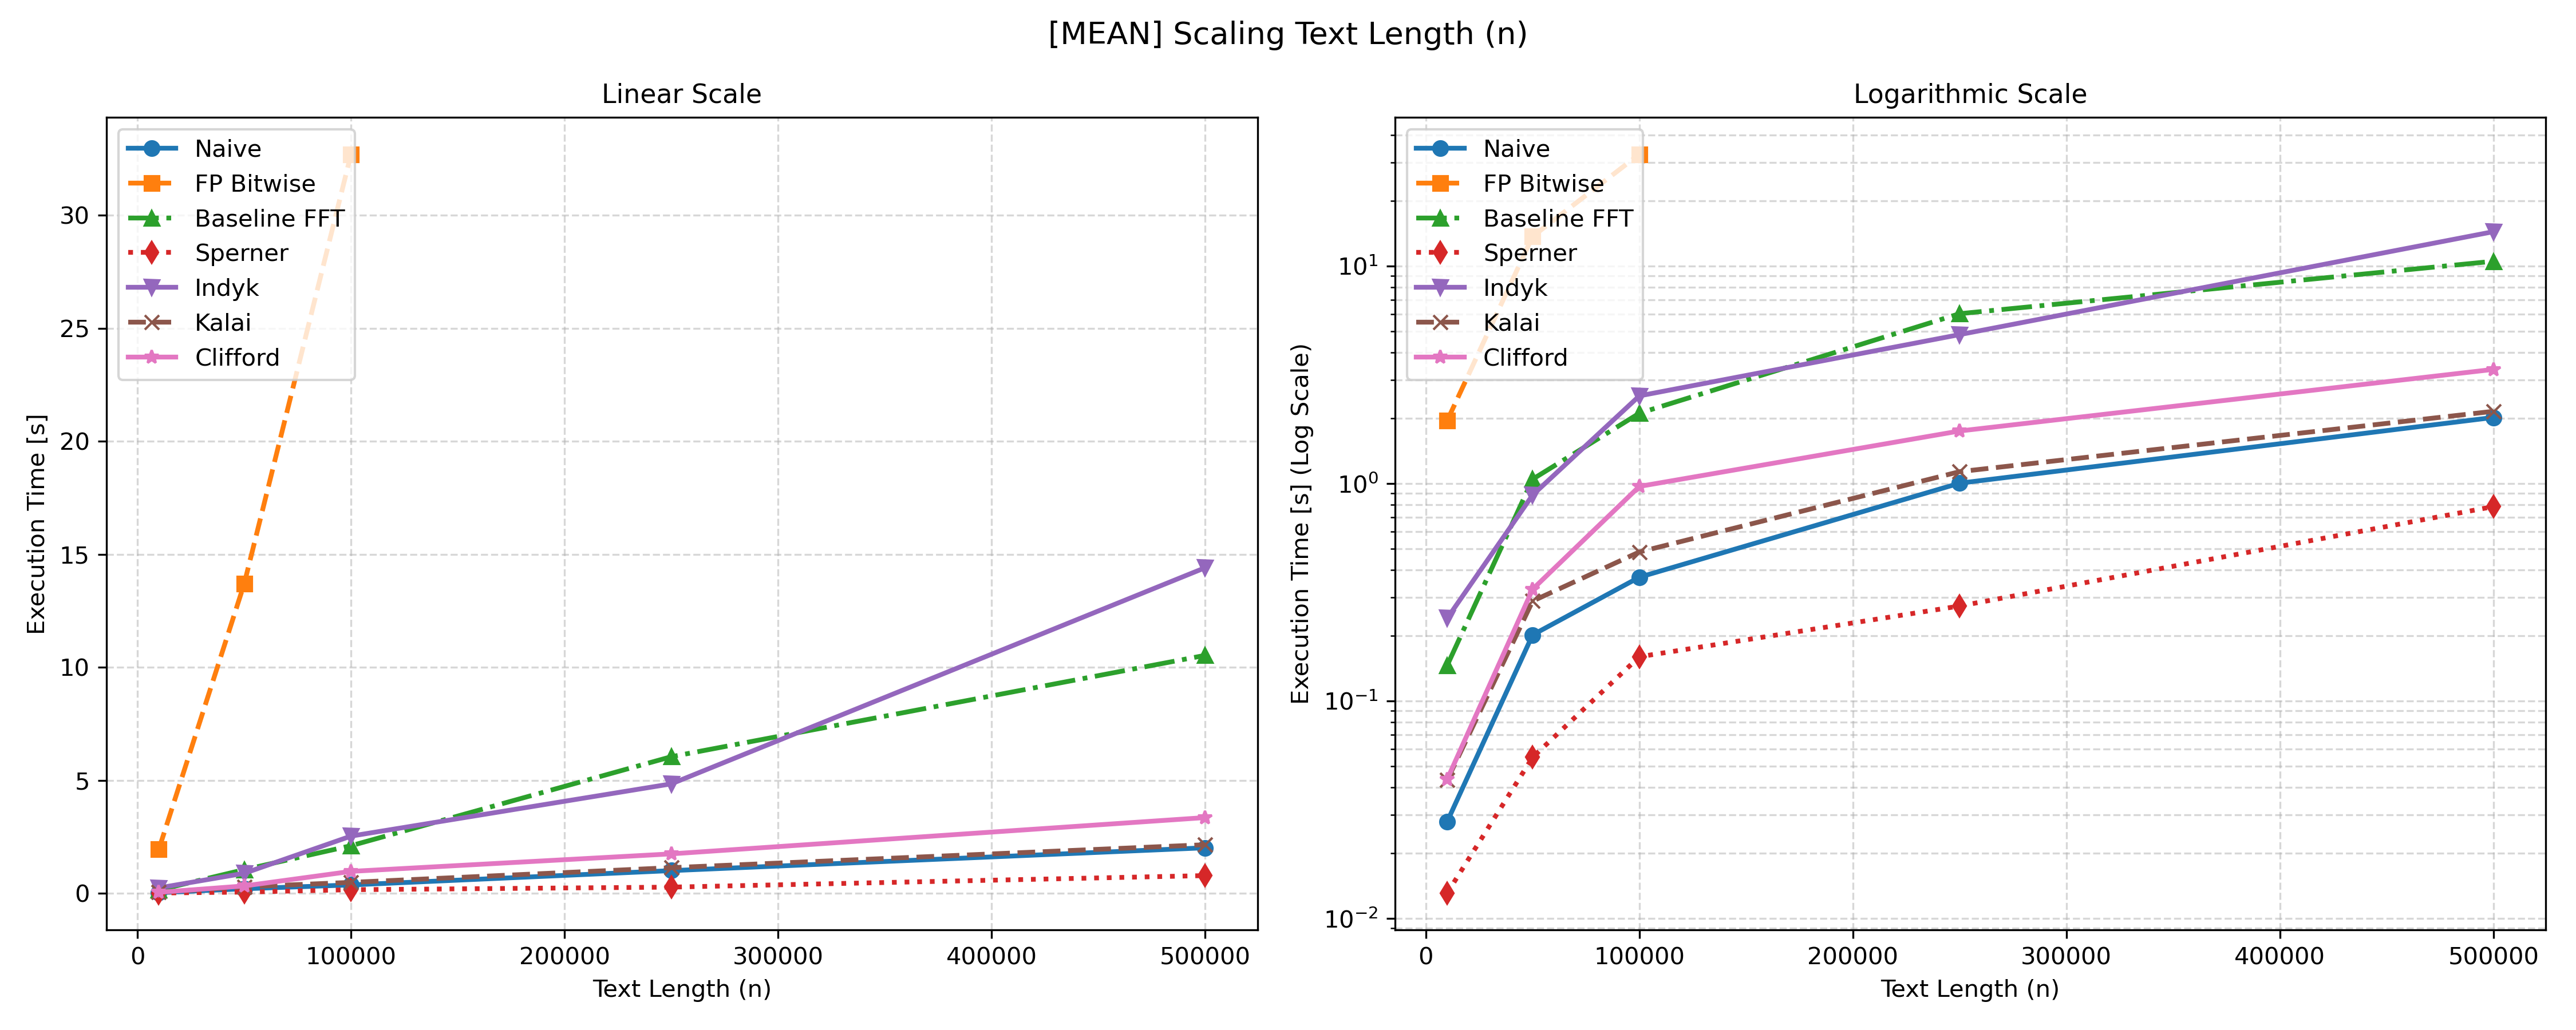
\includegraphics[width=\textwidth]{images/mean_plot_n.png}
    \caption{Scaling Text Length ($n$) under Average-Case conditions.}
    \label{fig:mean_n}
\end{figure}

Conversely, under worst-case inputs, every alignment forces the inner loop to scan through $m-1$ matching characters. As shown in Figure \ref{fig:worst_n}, the runtime increases drastically from $20.11$ seconds at $n=10000$ to over $366$ seconds at $n=100000$, after which it is safely omitted. This forms a sharp parabolic curve that confirms the exact $\mathcal{O}(nm)$ worst-case behavioral trap.

\begin{figure}[H]
    \centering
    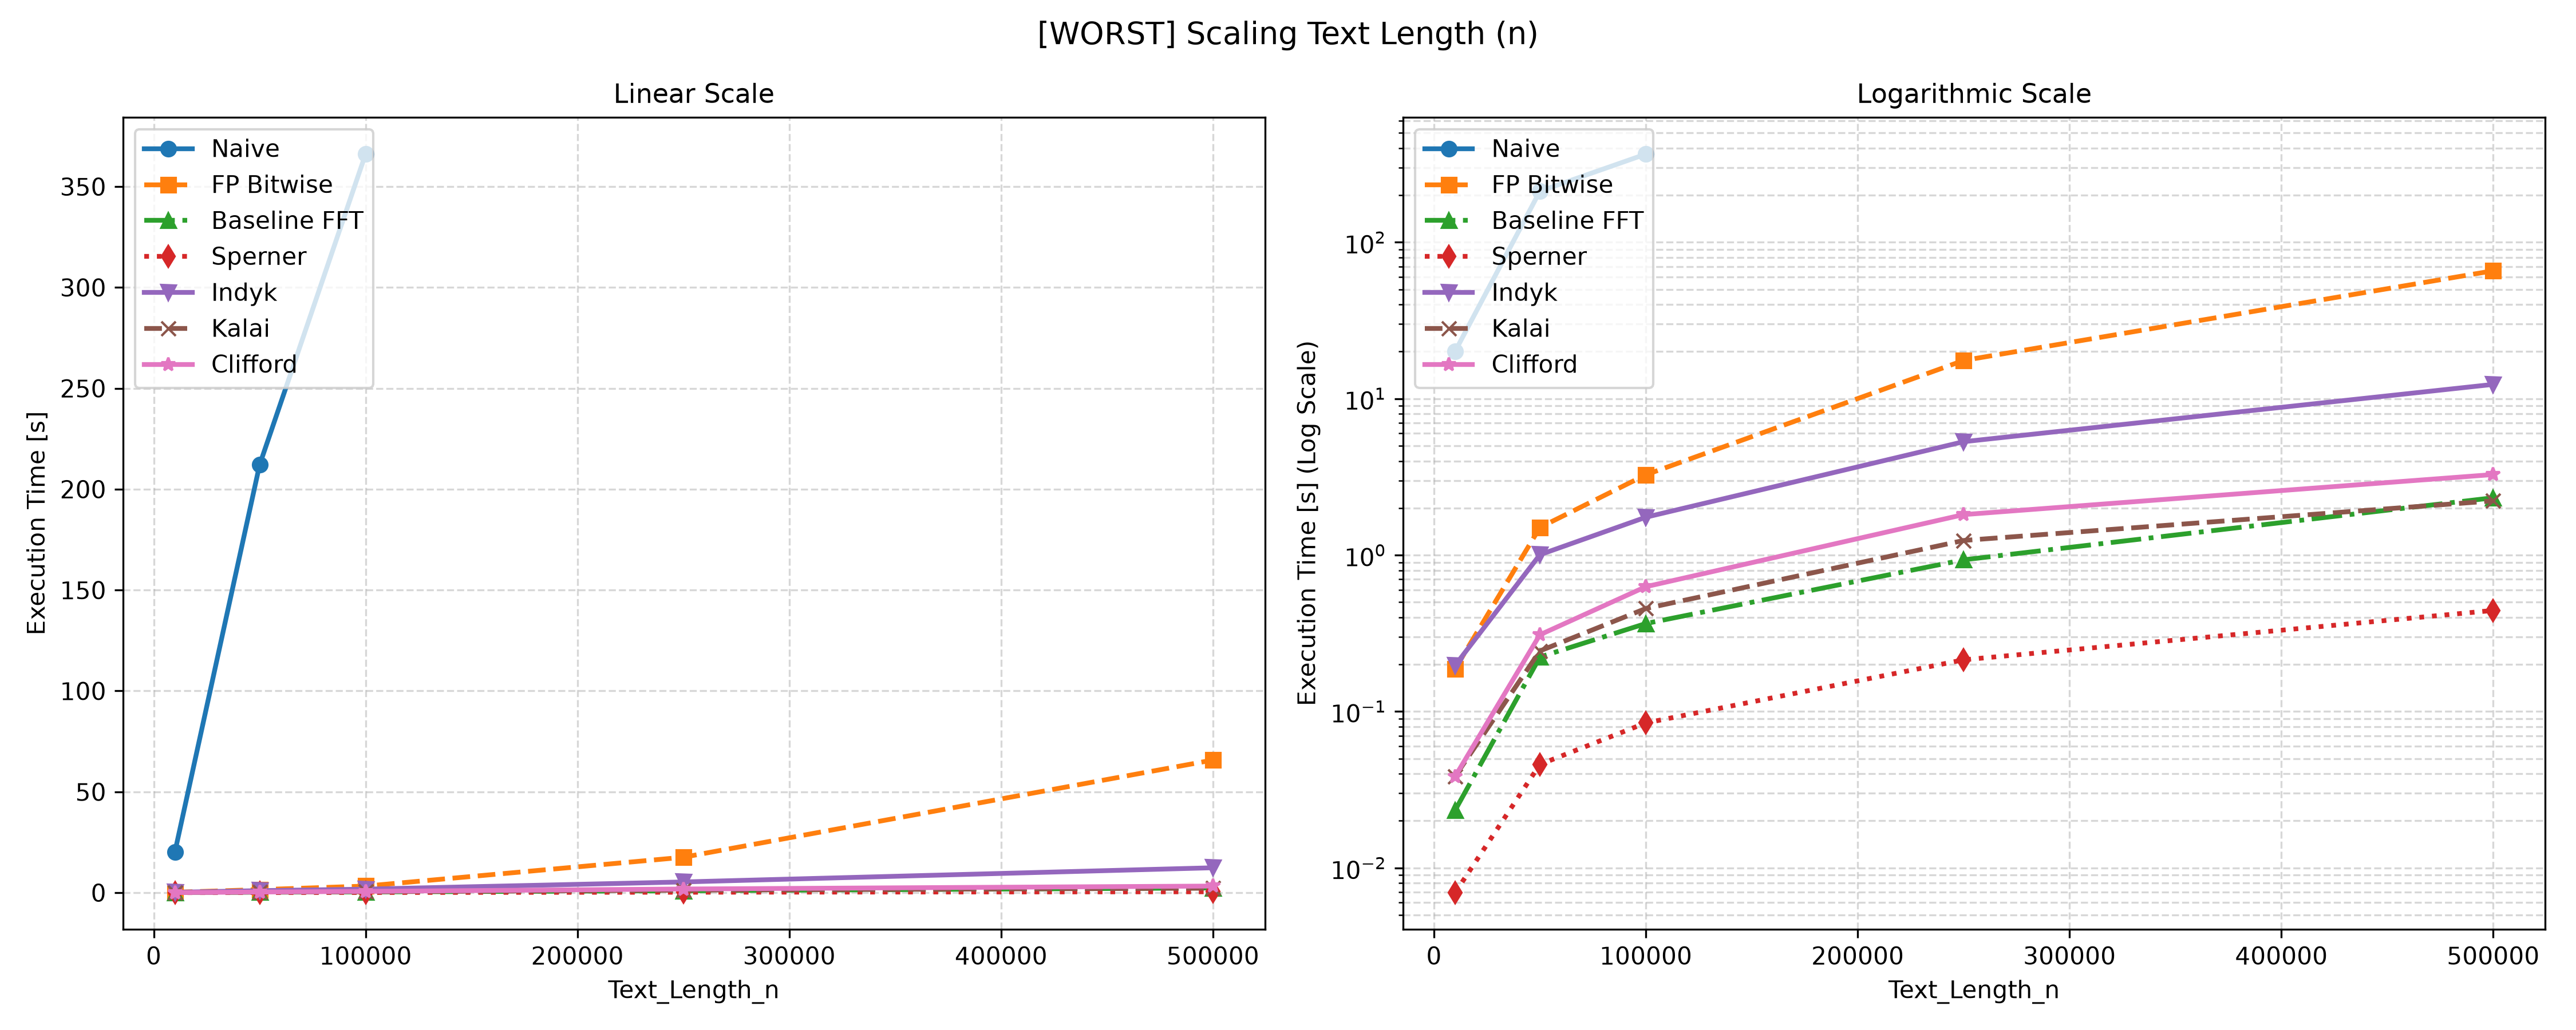
\includegraphics[width=\textwidth]{images/worst_plot_n.png}
    \caption{Scaling Text Length ($n$) under Worst-Case conditions.}
    \label{fig:worst_n}
\end{figure}

The structural degradation when scaling the pattern length $m$ (while holding the text length constant) fully mirrors the breakdown observed when scaling $n$. As shown in Figures \ref{fig:mean_m} and \ref{fig:worst_m}, increasing the pattern length matches the symmetric nature of the $\mathcal{O}(nm)$ worst-case boundary, while average-case execution remains mostly flat for the brute-force approach.

\begin{figure}[H]
    \centering
    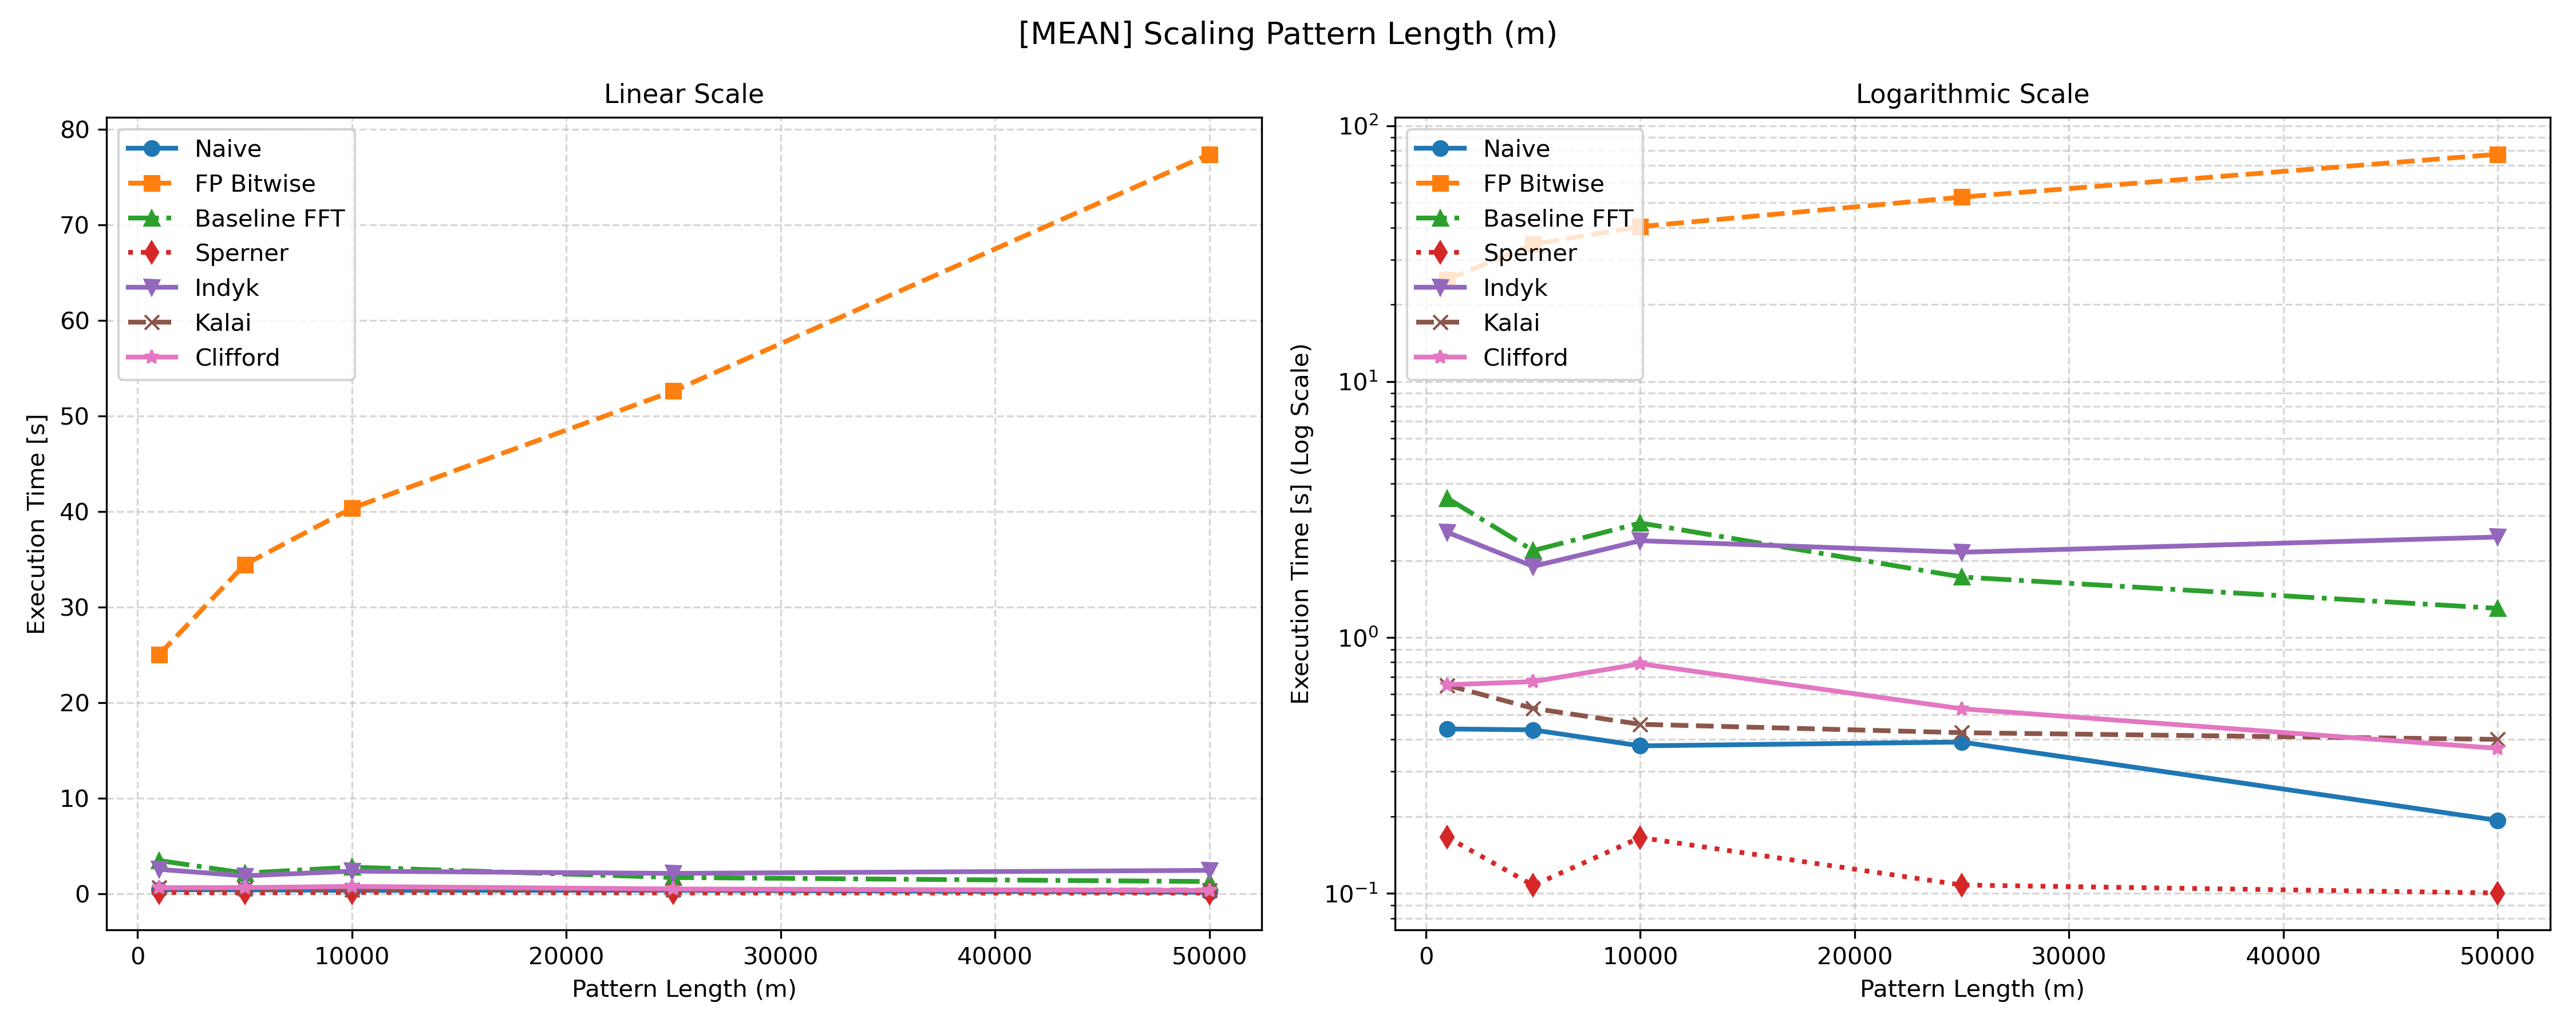
\includegraphics[width=\textwidth]{images/mean_plot_m.png}
    \caption{Scaling Pattern Length ($m$) under Average-Case conditions.}
    \label{fig:mean_m}
\end{figure}

\begin{figure}[H]
    \centering
    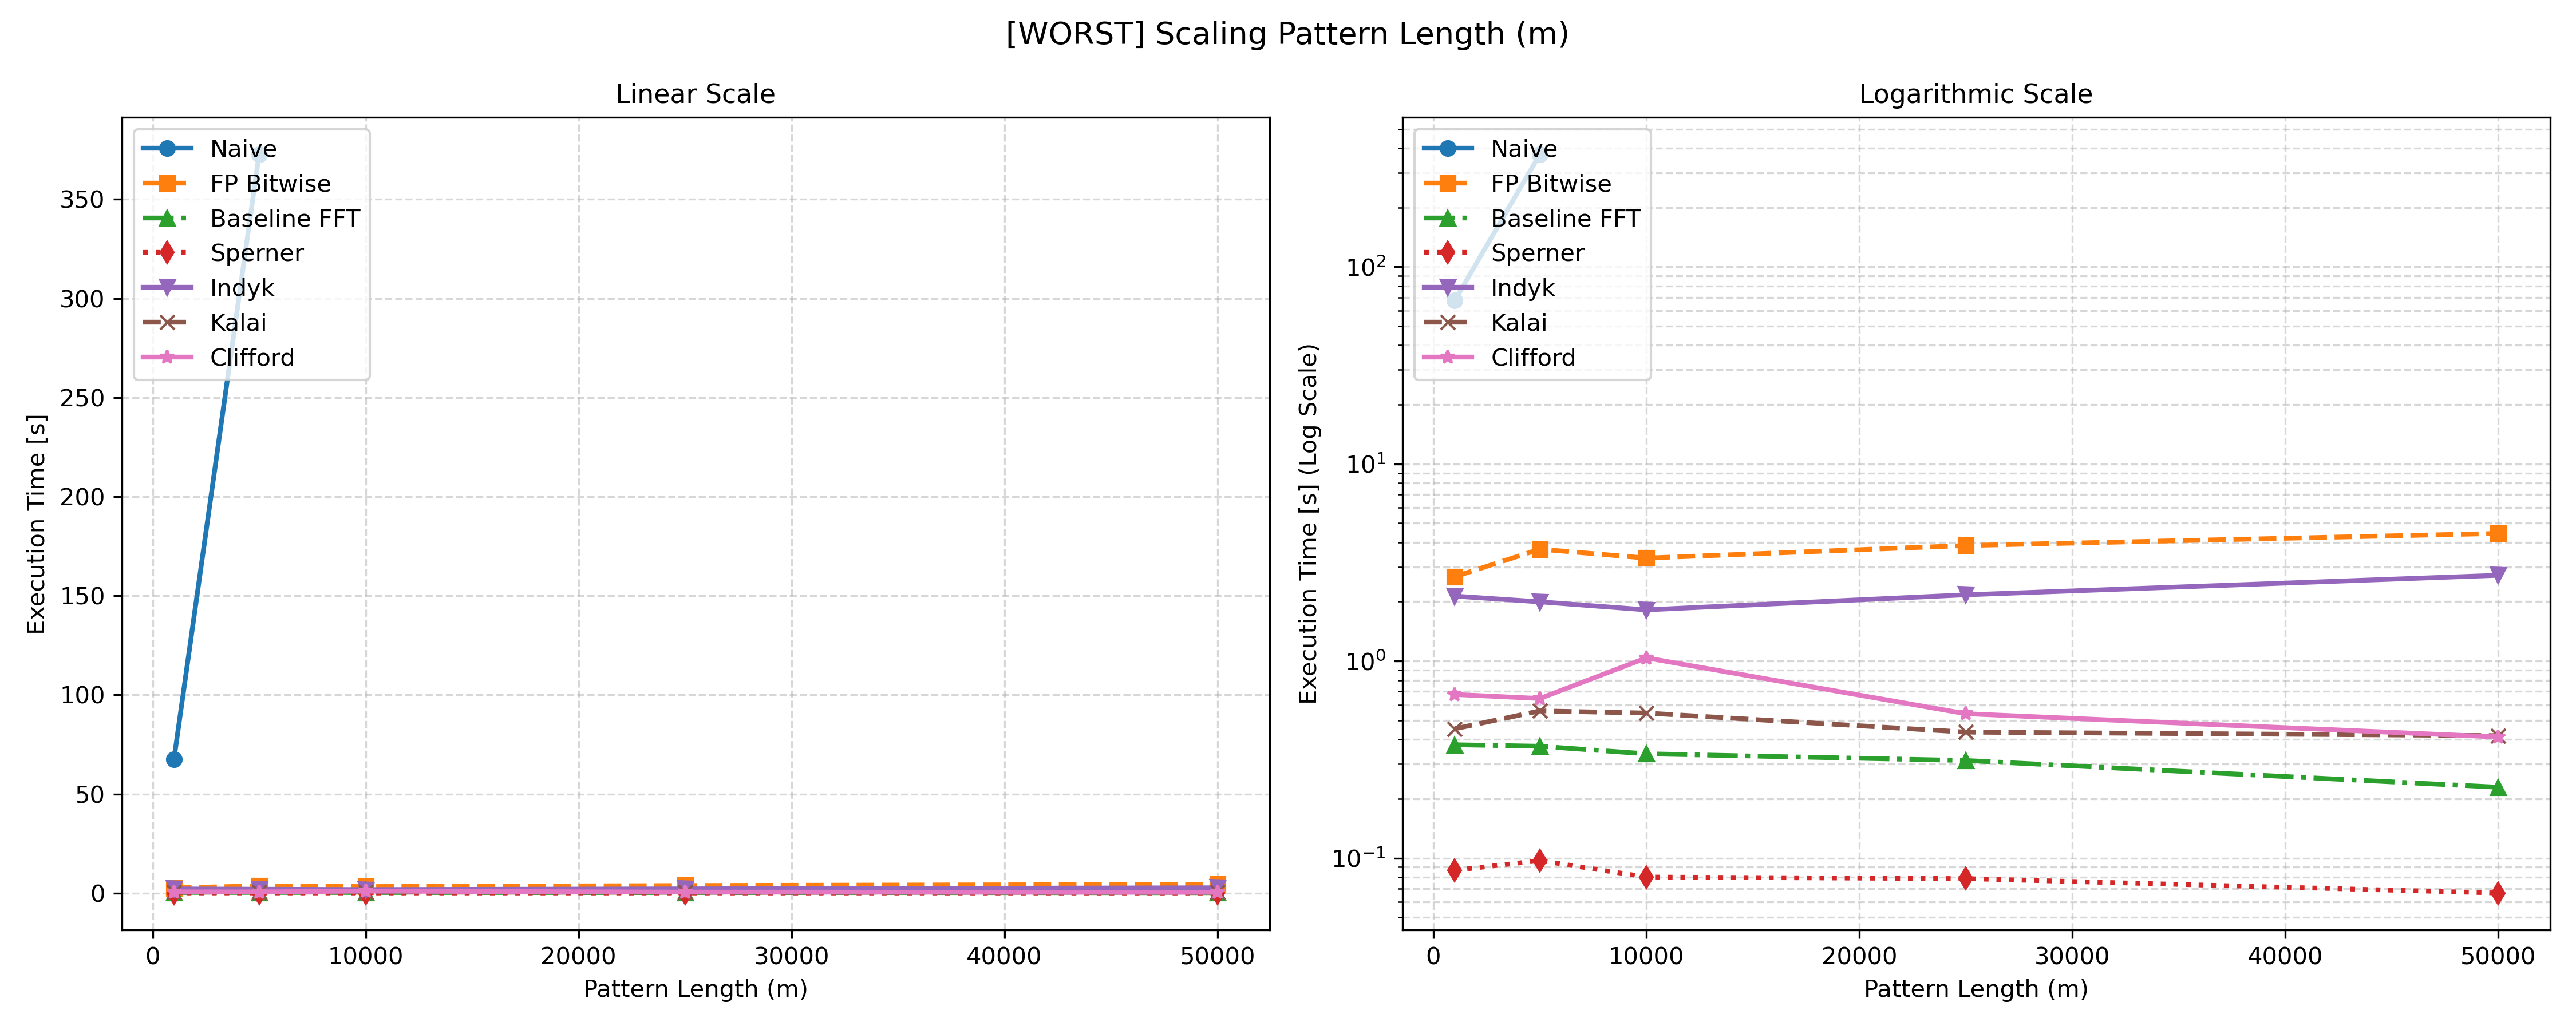
\includegraphics[width=\textwidth]{images/worst_plot_m.png}
    \caption{Scaling Pattern Length ($m$) under Worst-Case conditions.}
    \label{fig:worst_m}
\end{figure}

\section{Fischer-Paterson Bottleneck}
The Fischer-Paterson algorithm packs characters into large integers using bit shifts. The execution time depends heavily on the alphabet cardinality $|\Sigma|$ and the bit-length of the integer representations.

In the average-case test scaling the alphabet size (Figure \ref{fig:mean_sigma}), the presence of unique symbols forces the algorithm to execute Karatsuba multiplications over extremely large integers. This generates a significant polynomial performance degradation, where execution time surges to over $150$ seconds for an alphabet of $64$ symbols. 

\begin{figure}[H]
    \centering
    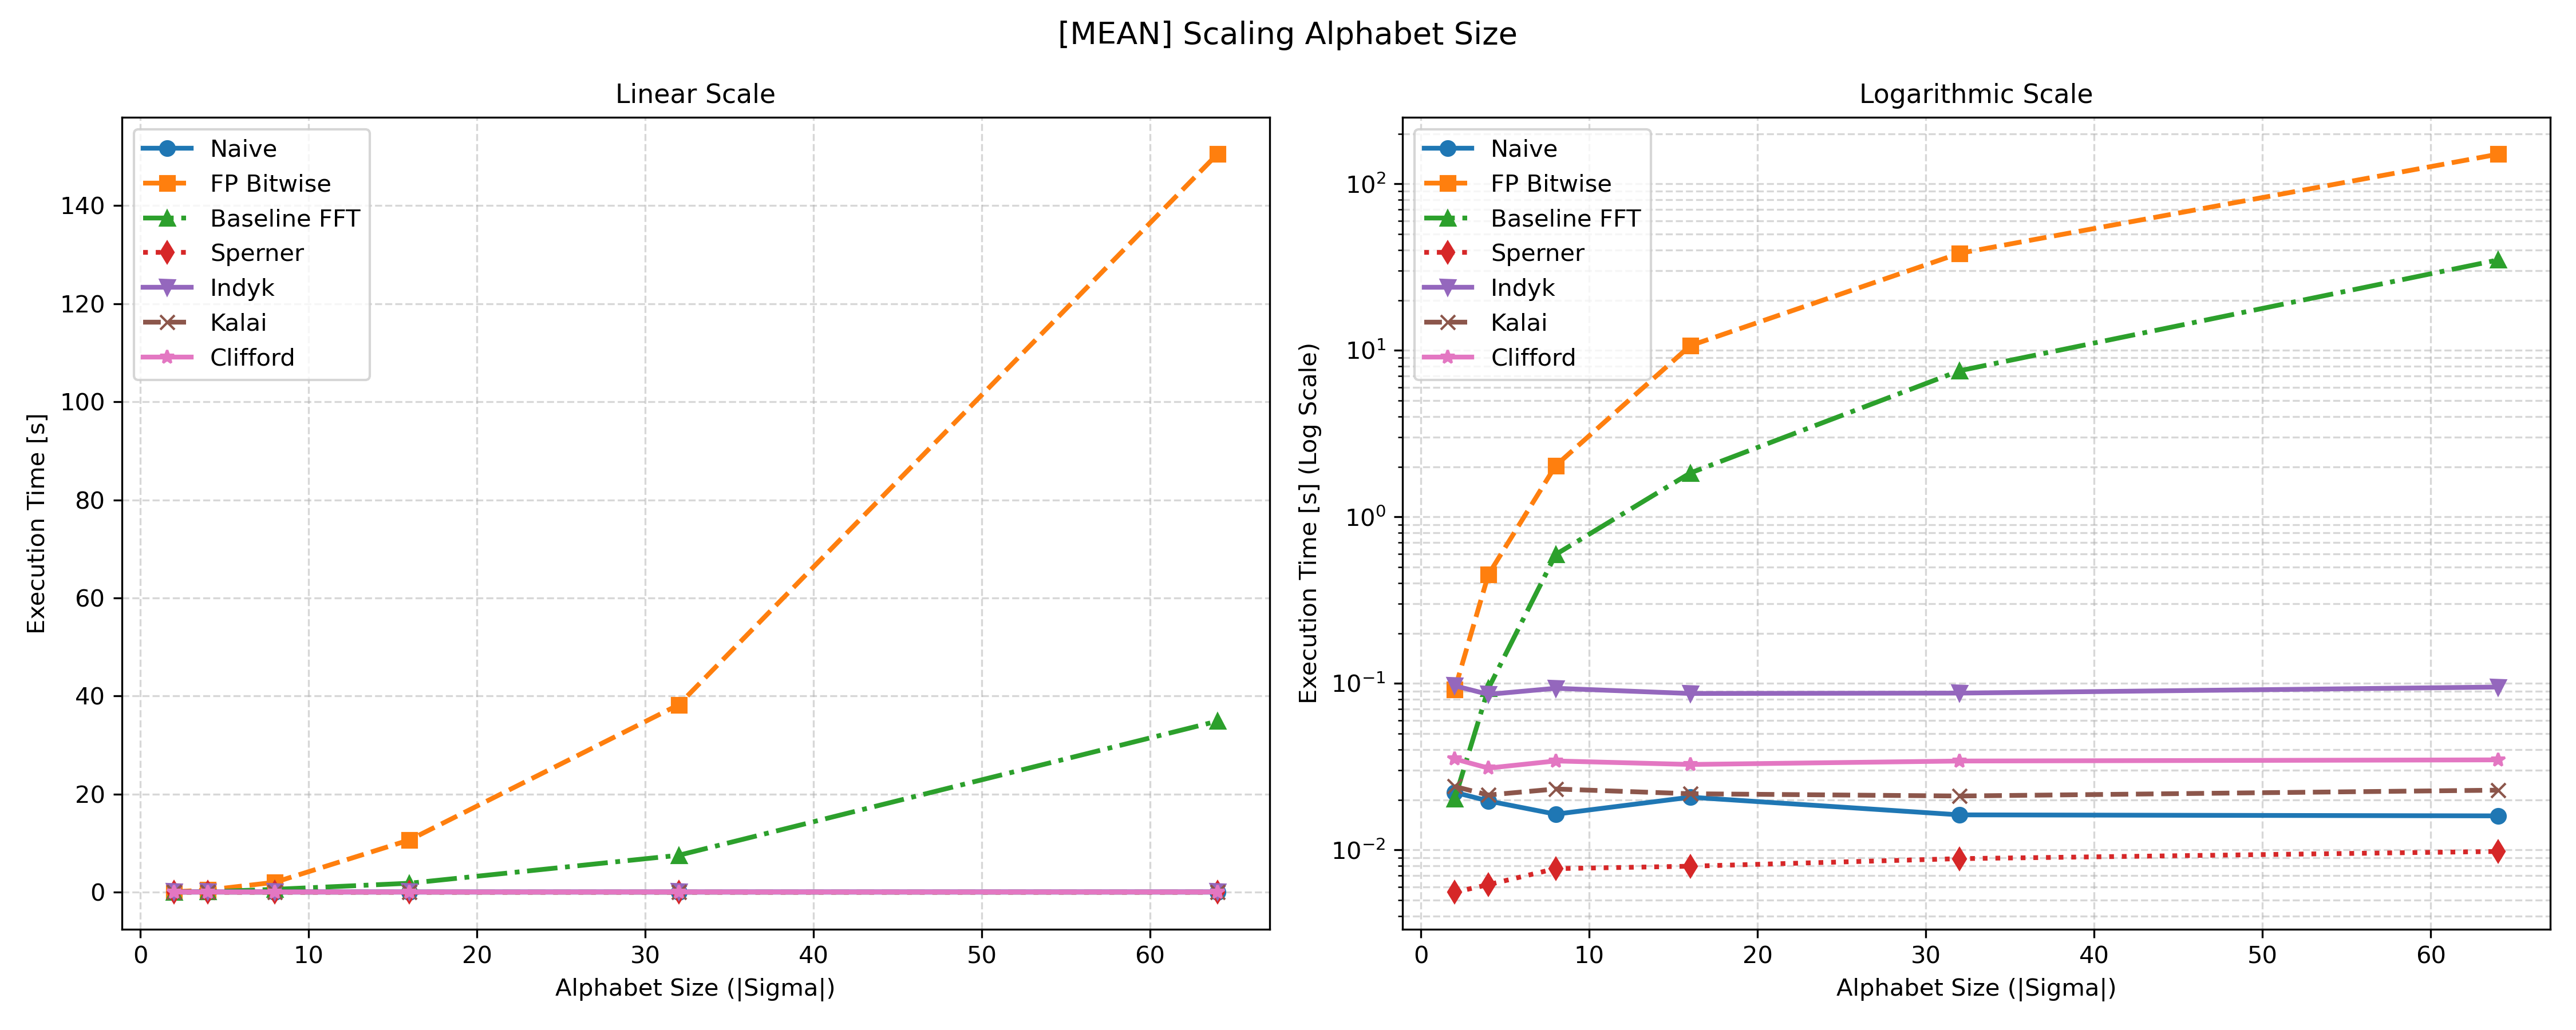
\includegraphics[width=\textwidth]{images/mean_plot_sigma.png}
    \caption{Scaling Alphabet Size ($|\Sigma|$) under Average-Case conditions.}
    \label{fig:mean_sigma}
\end{figure}

This exponential rise is uniquely bound to the FP Bitwise approach. As shown in the worst-case scaling (Figure \ref{fig:worst_sigma}), where the text is predominantly composed of a single repeating character, the arbitrary-precision multiplication completes significantly faster due to the lower variance in bits. More importantly, both figures firmly confirm that all modern FFT-based convolutions remain entirely decoupled from alphabet size constraints.

\begin{figure}[H]
    \centering
    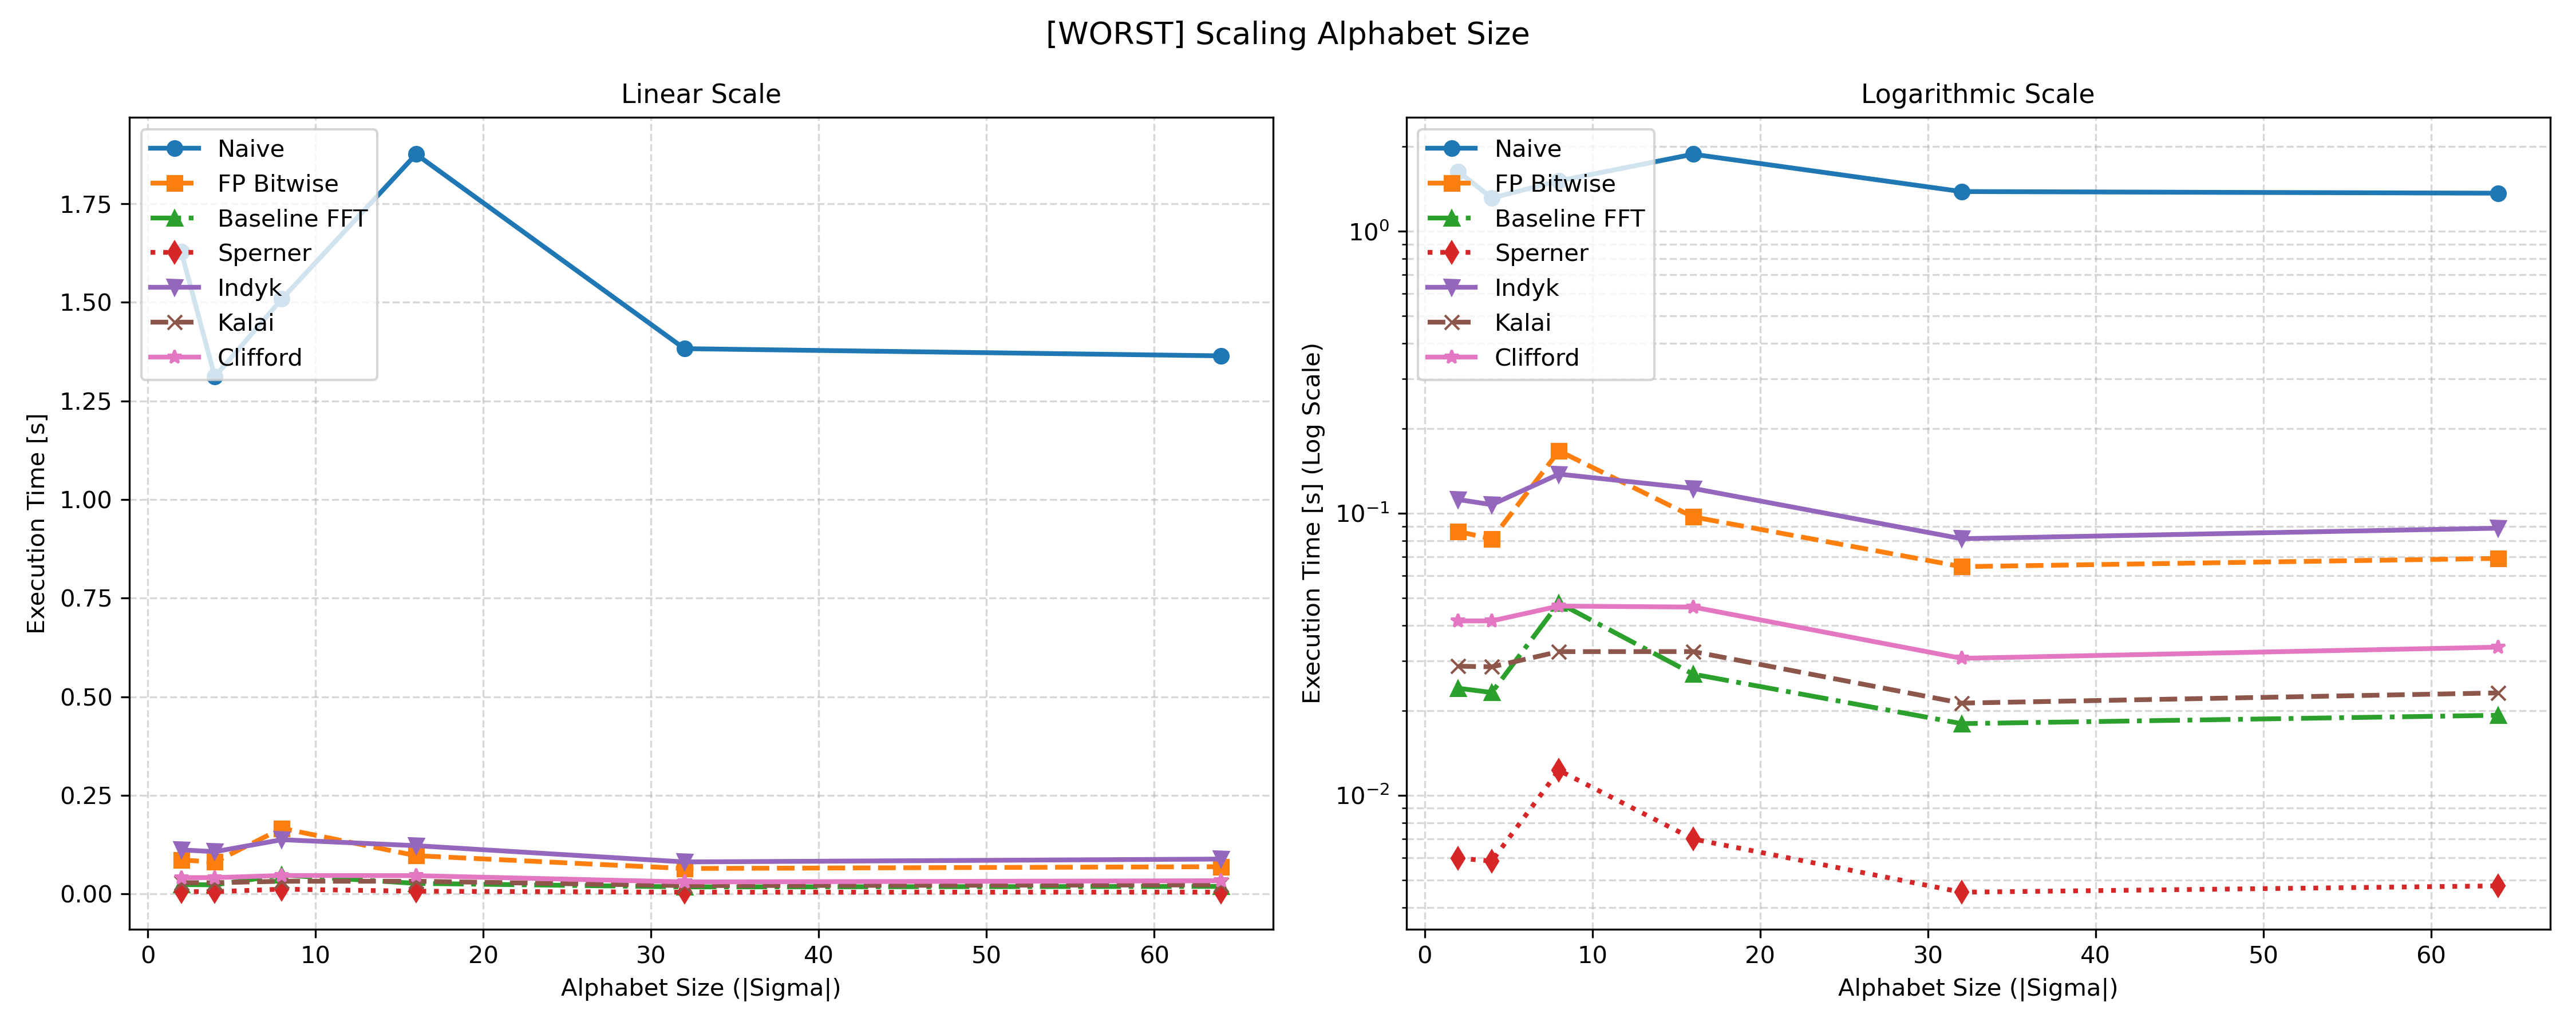
\includegraphics[width=\textwidth]{images/worst_plot_sigma.png}
    \caption{Scaling Alphabet Size ($|\Sigma|$) under Worst-Case conditions.}
    \label{fig:worst_sigma}
\end{figure}

\section{Constant Factors: Kalai, Indyk, and Clifford-Clifford}
Indyk, Kalai, and Clifford-Clifford all exhibit theoretically optimal or near-optimal asymptotic complexities. However, the benchmark plots reveal practical differences driven by their internal theoretical constant factors. 

For a large-scale text of length $n=500000$, Indyk takes $14.40$ seconds, Clifford-Clifford completes in $3.35$ seconds, and Kalai finishes natively in only $2.15$ seconds. 

This performance hierarchy aligns perfectly with their underlying algebraic structures:
\begin{itemize}
    \item \textbf{Kalai (Probabilistic Optimal):} Requires exactly two forward FFTs and two inverse FFTs per search ($C_{\text{Kalai}} = 4 \cdot \mathcal{F}(L)$). This light constant factor makes it the fastest among the advanced convolution algorithms, though it inherently carries a mathematically bounded $\mathcal{O}(1/n)$ error risk.
    \item \textbf{Clifford-Clifford (Deterministic Optimal):} Evaluates the exact Euclidean distance using exactly three FFT passes on squared and cubed numerical arrays. Generating these high-power algebraic vectors and managing block-overlaps introduces a slightly heavier constant factor than Kalai, but it successfully eliminates the probabilistic error risk, making it the most efficient purely deterministic solution.
    \item \textbf{Indyk (Randomized Projections):} To keep the false-positive rate sufficiently low, it performs $d = c \cdot \log_2(n)$ independent projection dimensions. For large text inputs, this requires generating multiple independent trials and executing dozens of physical FFT operations sequentially. This severely penalizes the algorithm's practical runtime despite its theoretical $\mathcal{O}(n \log n)$ boundary.
\end{itemize}

\section{Proportional Asymptotic Scaling}
To directly observe theoretical boundaries, the proportional scaling test continuously increases the pattern length as $m = 0.1n$. This forces the algorithmic product $n \cdot m$ to grow quadratically, while $\mathcal{O}(n \log n)$ grows marginally faster than linearly. 

As captured in Figure \ref{fig:prop_nm}, the \textsc{Naive} algorithm forms a steep parabolic trajectory, reaching over $170$ seconds at $n=50000$. Meanwhile, the FFT-based algorithms appear completely flat on the linear scale. The logarithmic right panel reveals their true logarithmic progression, fitting the algebraic scalability proofs established by Kalai, Indyk, and Clifford-Clifford. Both Kalai and Clifford-Clifford finish in roughly $3$ seconds at $n=400000$, maintaining nearly parallel trajectories that match their tight $\mathcal{O}(n \log m)$ bounds.

\begin{figure}[H]
    \centering
    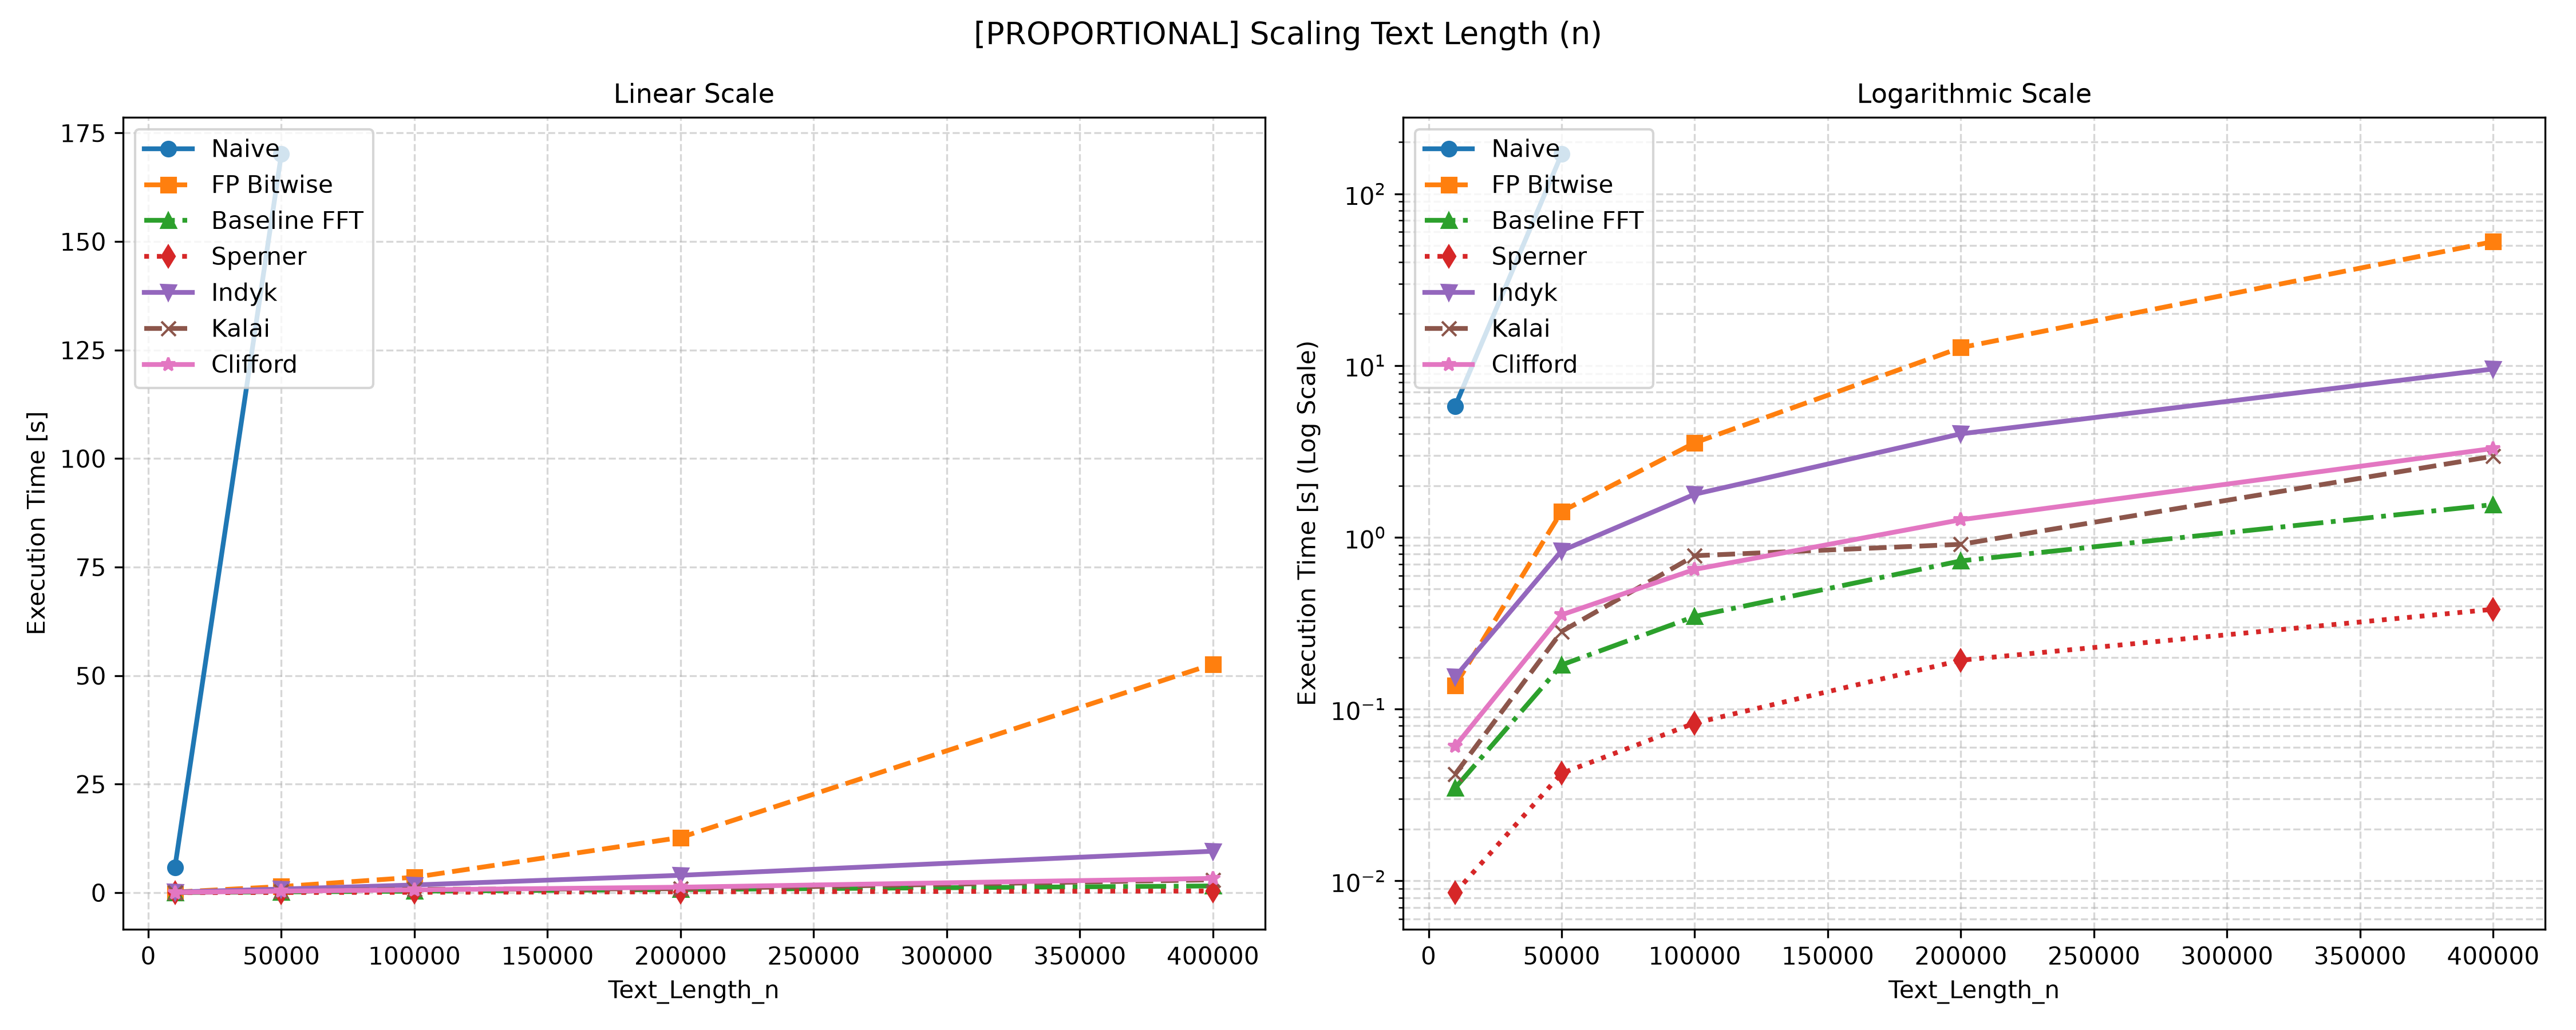
\includegraphics[width=\textwidth]{images/proportional_plot_nm.png}
    \caption{Proportional Scale Test proving $\mathcal{O}(n^2)$ vs $\mathcal{O}(n \log n)$ bounds.}
    \label{fig:prop_nm}
\end{figure}
\section{Wildcard Saturation}
The wildcard saturation experiment (Figure \ref{fig:density}) evaluates algorithm behavior as the wildcard density $p$ scales from $0\%$ to $50\%$. 

For the \textsc{Naive} algorithm, the execution time nearly doubles as the wildcard density grows (scaling from roughly $0.35$ to $0.60$ seconds). While this difference appears minimal on the macro scale, it exposes a fundamental structural vulnerability. Because the wildcard symbol mathematically guarantees a local match, a higher density prevents the algorithm's inner loop from breaking early upon encountering a mismatch. Consequently, the algorithm is forced to scan deeper into the pattern at every shift, directly increasing the total number of character comparisons.

\begin{figure}[H]
    \centering
    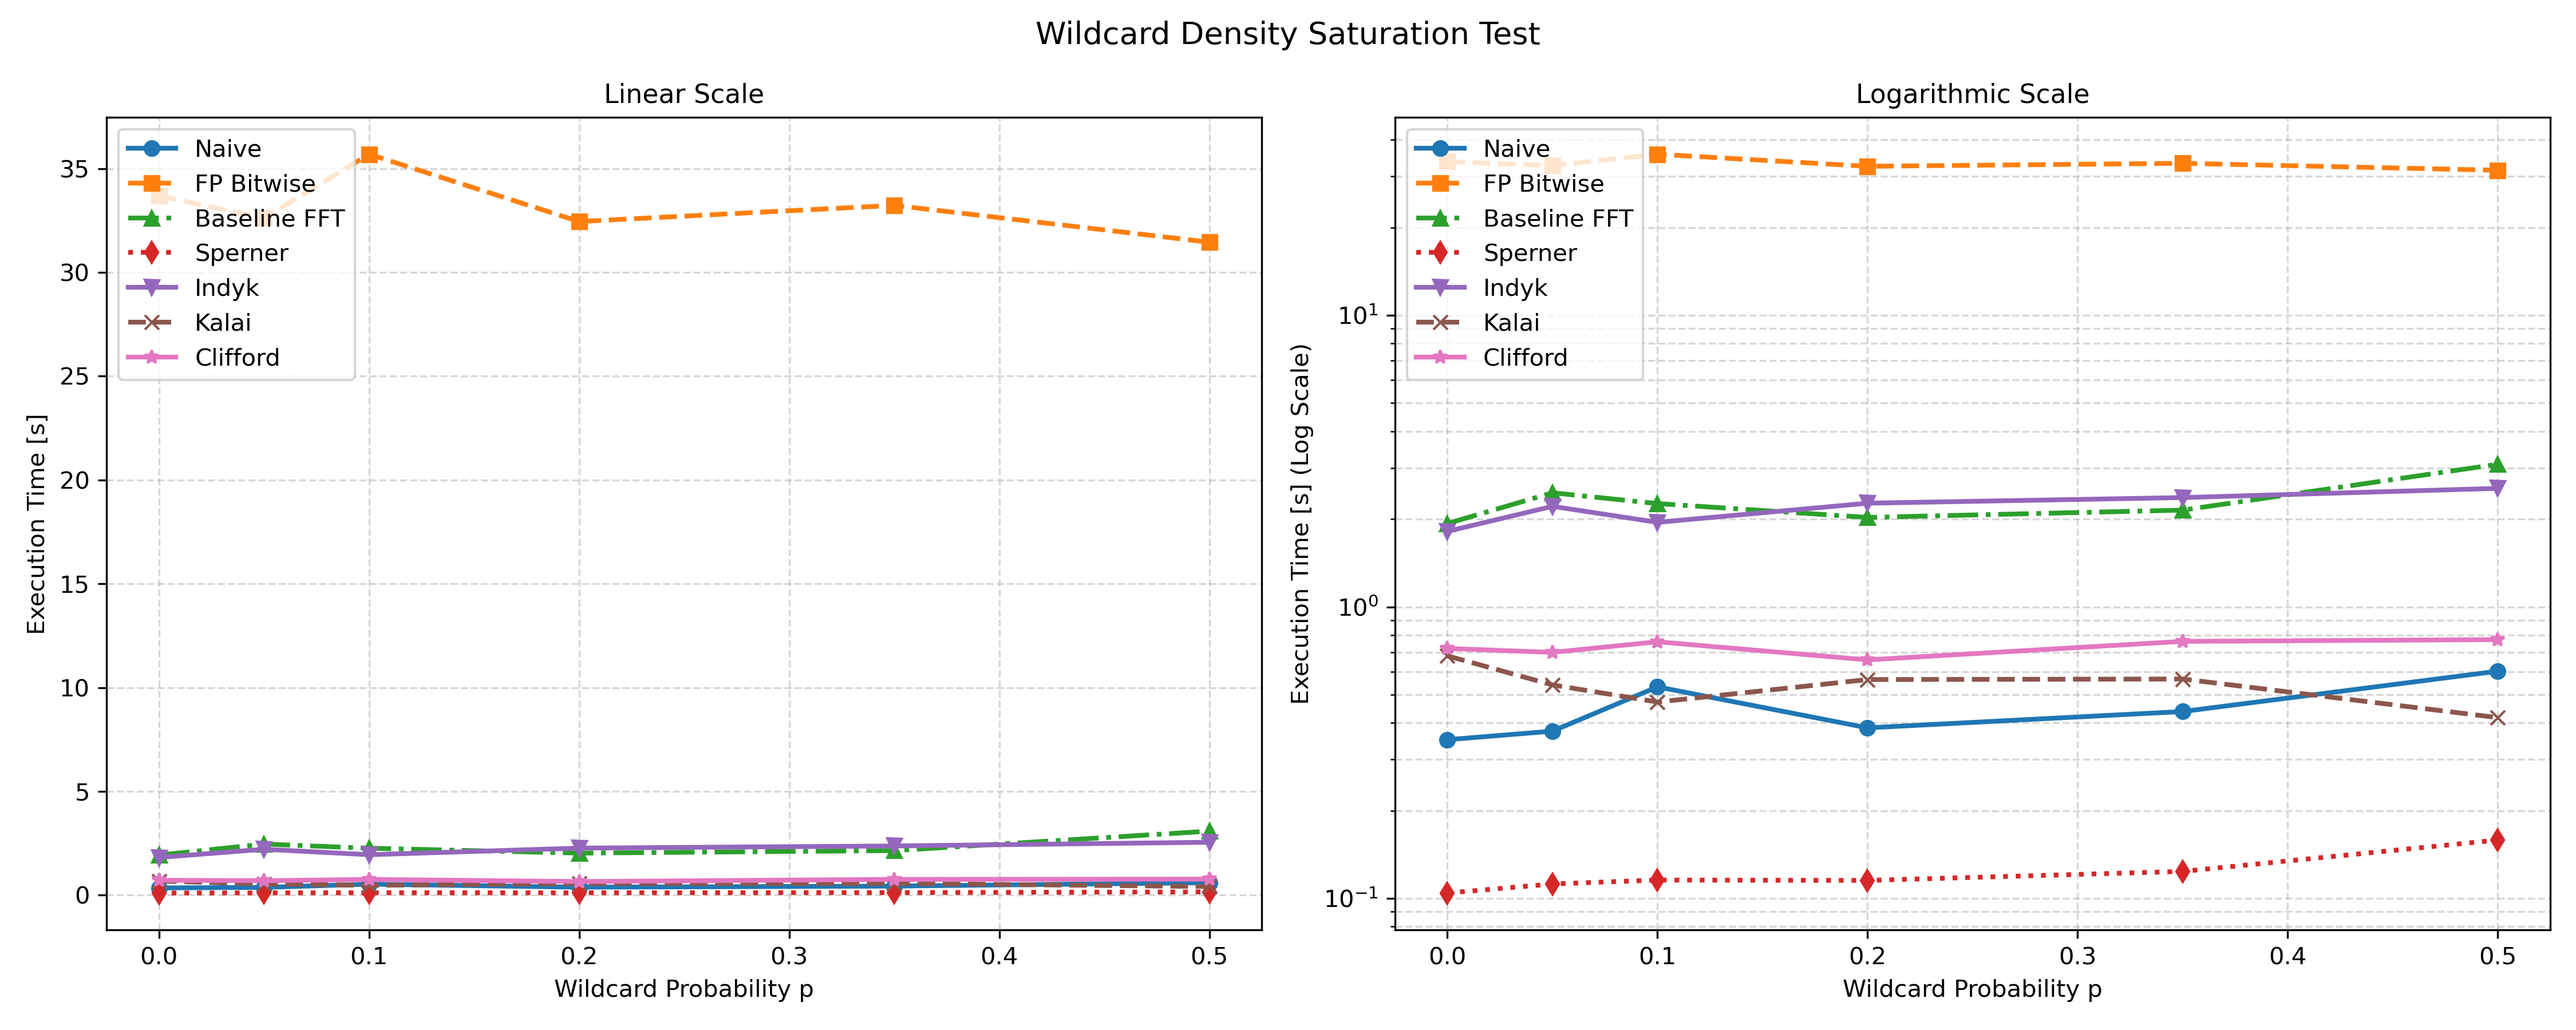
\includegraphics[width=\textwidth]{images/plot_wildcard_density.png}
    \caption{Wildcard Density Saturation Test.}
    \label{fig:density}
\end{figure}

In contrast, all convolution-based approaches remain stable because the required vector operations and FFT transforms are identical regardless of the input characters. With the array dimensions and the number of complex multiplications remaining constant, the presence of wildcards does not affect their execution speed.